%%%%%%%%%%%%%%%%%%%%%%%%%%%%%%%%%%%%%%%%%%%%%%%%%%%%%%%%%%%%%%%%%%%%%%%%%%%%%%%%%
%%
%% Fig 1: Comorbidity matrix
%%
%%%%%%%%%%%%%%%%%%%%%%%%%%%%%%%%%%%%%%%%%%%%%%%%%%%%%%%%%%%%%%%%%%%%%%%%%%%%%%%%%
%
\begin{figure}[!tbp]
\centering
%
\includegraphics[width=\textwidth]{\floatRelativePath/plthtmp_disease_comorbidity_matrix.py/corr_inkscape.png}
%
\caption{Trait distance based on the Spearman correlation of colocalized eQTL beta values for different gene and samples.}
\label{fig:gwas_distance}
%
\end{figure}

%%%%%%%%%%%%%%%%%%%%%%%%%%%%%%%%%%%%%%%%%%%%%%%%%%%%%%%%%%%%%%%%%%%%%%%%%%%%%%%%
%
% Tab 1: Winner eQTLs
%
%%%%%%%%%%%%%%%%%%%%%%%%%%%%%%%%%%%%%%%%%%%%%%%%%%%%%%%%%%%%%%%%%%%%%%%%%%%%%%%%

% full size table is table
\begin{table}[!tbp]
\centering
\scriptsize
%\hline
\csvreader[separator=tab,
tabular=crclcp{0.4\textwidth},
head,
table head=\bfseries Chrom. & \bfseries Pos (hg38) & \bfseries Cytoband & \bfseries RSID & \bfseries Marker & \bfseries GWAS Categories\\\hline,
]{\floatRelativePath/cmpt_count_per_rsid.py/count_per_rsid_gwas_ms.tsv}{}% use head of csv as column names
{\csvcoli\ & \csvcolii\ & \csvcoliii\ & \csvcoliv\ & \csvcolv\ & \csvcolvi}% specify your coloumns here
%\hline
%
\vspace{15pt}
%
\caption{eQTLs involved in four GWAS categories. The gene marker is the eQTL gene with the highest PubMed publication count.}
\label{tab:pleitropic_variants}
\end{table}

%%%%%%%%%%%%%%%%%%%%%%%%%%%%%%%%%%%%%%%%%%%%%%%%%%%%%%%%%%%%%%%%%%%%%%%%%%%%%%%%
%
% Tab 2: Winner regions
%
%%%%%%%%%%%%%%%%%%%%%%%%%%%%%%%%%%%%%%%%%%%%%%%%%%%%%%%%%%%%%%%%%%%%%%%%%%%%%%%%

% full size table is table
\begin{table}[!tbp]
\centering
\scriptsize
%\hline
\csvreader[
separator=tab,
tabular=p{0.02\textwidth}p{0.09\textwidth}p{0.09\textwidth}p{0.05\textwidth}p{0.09\textwidth}p{0.09\textwidth}p{0.45\textwidth},
head,
table head=\bfseries Chr. & \bfseries Start & \bfseries End & \bfseries Cytob. & \bfseries Pleio RSID & \bfseries Pleio pos. & \bfseries GWAS Categories\\\hline,
]{\floatRelativePath/cmpt_pleiotropic_regions.py/100000/region_window_ms.tsv}{}% use head of csv as column names
{\csvcoli\ & \csvcolv\ & \csvcolvi\ & \csvcoliv\ & \csvcolii\ & \csvcoliii\ & \csvcolvii}% specify your coloumns here
%\hline
%
\vspace{15pt}
\caption{Pleiotropic regions involving 6 or more GWAS classes. These regions were built with a sliding window of 1e5 nt. Genomic coordinates are given for the hg38 assembly.}\label{tab:pleiotropic_regions}
\end{table}

%%%%%%%%%%%%%%%%%%%%%%%%%%%%%%%%%%%%%%%%%%%%%%%%%%%%%%%%%%%%%%%%%%%%%%%%%%%%%%%%%
%%
%% Fig 2: Length histogram of regions
%%
%%%%%%%%%%%%%%%%%%%%%%%%%%%%%%%%%%%%%%%%%%%%%%%%%%%%%%%%%%%%%%%%%%%%%%%%%%%%%%%%%
%
% \begin{figure}[!tbp]
% \centering
% %
% \begin{subfigure}[]{.33\textwidth}
% \textbf{a}
% \\
% \includegraphics[width=\textwidth]{\floatRelativePath/cmpt_pleiotropic_regions.py/regions_100000_length_hist.png}
% \end{subfigure}
% %
% \begin{subfigure}[]{.33\textwidth}
% \textbf{b}
% \\
% \includegraphics[width=\textwidth]{\floatRelativePath/pltbar_pleiotropic_regions_cumsum.py/pltbar_regions_cumsum.png}
% \end{subfigure}
% %
% \caption{Analysis of pleiotropic regions. \textbf{a}, Length distribution of pleiotropic regions. \textbf{b}, Cumulative sum ordered inversely with the number of GWAS classes.} \label{fig:pleiotropy_region_distribution}
% \end{figure}
%
%%%%%%%%%%%%%%%%%%%%%%%%%%%%%%%%%%%%%%%%%%%%%%%%%%%%%%%%%%%%%%%%%%%%%%%%%%%%%%%%%
%%
%% Fig 3: Histograms variants vs GWAS, eGene and eTissues
%%
%%%%%%%%%%%%%%%%%%%%%%%%%%%%%%%%%%%%%%%%%%%%%%%%%%%%%%%%%%%%%%%%%%%%%%%%%%%%%%%%%
%
\begin{figure}[!tbp]
\centering
%
\begin{subfigure}[]{.32\textwidth}
\textbf{a}
\\
\includegraphics[width=\textwidth]{\floatRelativePath/plthst_gwas_egene_etissue.py/hist_gwas.png}
\end{subfigure}
%
\begin{subfigure}[]{.32\textwidth}
\textbf{b}
\\
\includegraphics[width=\textwidth]{\floatRelativePath/plthst_gwas_egene_etissue.py/hist_egene.png}
\end{subfigure}
%
\begin{subfigure}[]{.32\textwidth}
\textbf{c}
\\
\includegraphics[width=\textwidth]{\floatRelativePath/plthst_gwas_egene_etissue.py/hist_etissue.png}
\end{subfigure}
%
\caption{Percentage of colocalized eQTL/GWAS variants with different number of GWAS classes (\textbf{a}), eQTL genes
    (\textbf{b}) and eQTL tissues (\textbf{c}).} \label{fig:hist_gwas_egene_etissue}
\end{figure}

%%%%%%%%%%%%%%%%%%%%%%%%%%%%%%%%%%%%%%%%%%%%%%%%%%%%%%%%%%%%%%%%%%%%%%%%%%%%%%%%%
%%
%% Fig 4: Correlation between GWAS, genes and tissue counts
%%
%%%%%%%%%%%%%%%%%%%%%%%%%%%%%%%%%%%%%%%%%%%%%%%%%%%%%%%%%%%%%%%%%%%%%%%%%%%%%%%%%
%
\begin{figure}[!tbp]
\centering
%
\includegraphics[width=0.7\textwidth]{\floatRelativePath/cmpt_count_per_rsid.py/count_per_rsid_gwas_egene_etissue_corr.png}
%
\caption{Spearman correlation between the counts of GWAS classes, eQTL genes and eQTL tissues.}
\label{fig:correlation_counts}
%
\end{figure}

%%%%%%%%%%%%%%%%%%%%%%%%%%%%%%%%%%%%%%%%%%%%%%%%%%%%%%%%%%%%%%%%%%%%%%%%%%%%%%%%
%
% Fig 5: VEP consequences
%
%%%%%%%%%%%%%%%%%%%%%%%%%%%%%%%%%%%%%%%%%%%%%%%%%%%%%%%%%%%%%%%%%%%%%%%%%%%%%%%%

\begin{figure}[!tbp]
\centering
%
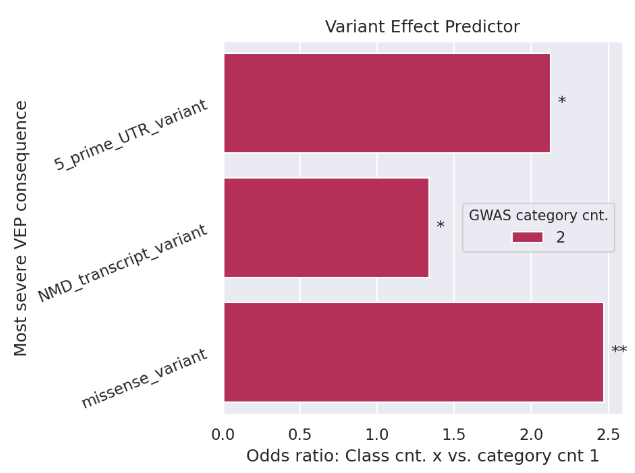
\includegraphics[width=\textwidth]{\floatRelativePath/pltbar_vep_consequence.py/vep.png}
%
\caption{Odds ratio of the variants annotated with given variant effect
predictor (VEP) consequence and given GWAS class count compared with non
pleiotropic variants with GWAS class count one. The significance is given for the
q-value with False discovery rate 5\%.}
\label{fig:vep_consequence}
%
\end{figure}

%%%%%%%%%%%%%%%%%%%%%%%%%%%%%%%%%%%%%%%%%%%%%%%%%%%%%%%%%%%%%%%%%%%%%%%%%%%%%%%%%
%%
%% Fig 6: Violin plots. eGenes, eTissues and gwas per variants
%%
%%%%%%%%%%%%%%%%%%%%%%%%%%%%%%%%%%%%%%%%%%%%%%%%%%%%%%%%%%%%%%%%%%%%%%%%%%%%%%%%%
%
\begin{figure}[!tbp]
\centering
%
\begin{subfigure}[]{.32\textwidth}
\textbf{a}
\\
\includegraphics[width=\textwidth]{\floatRelativePath/pltbar_x_per_variant_etissue_y_egene.py/plt.png}
\end{subfigure}
%
\begin{subfigure}[]{.32\textwidth}
\textbf{b}
\\
\includegraphics[width=\textwidth]{\floatRelativePath/pltbar_x_per_variant_egene_y_etissue.py/plt.png}
\end{subfigure}
%
%\begin{subfigure}[]{.32\textwidth}
%\textbf{c}
%\\
%\includegraphics[width=\textwidth]{\floatRelativePath/pltbar_x_per_variant_egene_etissue_y_gwas.py/plt.png}
%\end{subfigure}
%
\caption{Mean number of genes in eQTL-tissue pairs (\textbf{a}) and mean number of tissues in eQTL-gene pairs (\textbf{b}).} \label{fig:gwas_egene_etisue_per_variant}
%
\end{figure}

%%%%%%%%%%%%%%%%%%%%%%%%%%%%%%%%%%%%%%%%%%%%%%%%%%%%%%%%%%%%%%%%%%%%%%%%%%%%%%%%%
%%
%% Fig 7: TF count per GWAS class count
%%
%%%%%%%%%%%%%%%%%%%%%%%%%%%%%%%%%%%%%%%%%%%%%%%%%%%%%%%%%%%%%%%%%%%%%%%%%%%%%%%%%

\begin{figure}[!tbp]
\centering
%
\begin{subfigure}[]{.33\textwidth}
\textbf{a}
\\
\includegraphics[width=\textwidth]{\floatRelativePath/pltbox_x_per_rsid_y_remapnr.py/bxplt_remaptf_per_rsid_flank_10.png}
\end{subfigure}
%
\begin{subfigure}[]{.33\textwidth}
\textbf{b}
\\
\includegraphics[width=\textwidth]{\floatRelativePath/pltbar_x_per_variant_pleiotropy_y_remapcrm.py/remapcrm_flank10.png}
\end{subfigure}
%
\caption{Analysis of transcription factor binding.
\textbf{a}, Binding count of transcription factors in the region surrounding pleiotropic eQTLs with a radius of 50 bp as a function of the GWAS class count.
\textbf{b}, Odds ratio of eQTLs annotated as belonging to a cis regulatory modules vs. non-annotated.} \label{fig:freq_tf_per_variant}
%
\end{figure}

%%%%%%%%%%%%%%%%%%%%%%%%%%%%%%%%%%%%%%%%%%%%%%%%%%%%%%%%%%%%%%%%%%%%%%%%%%%%%%%%%
%%
%% Fig 8: beta and log pval
%%
%%%%%%%%%%%%%%%%%%%%%%%%%%%%%%%%%%%%%%%%%%%%%%%%%%%%%%%%%%%%%%%%%%%%%%%%%%%%%%%%%
%
%\begin{figure}[!tbp]
%\centering
%%
%\begin{subfigure}[]{.33\textwidth}
%\textbf{a}
%\\
%\includegraphics[width=\textwidth]{\floatRelativePath/pltbar_x_per_gwas_cat_y_beta.py/eqtl_beta.png}
%\end{subfigure}
%%
%\begin{subfigure}[]{.33\textwidth}
%\textbf{b}
%\\
%\includegraphics[width=\textwidth]{\floatRelativePath/pltbar_x_per_gwas_cat_y_beta.py/gwas_beta.png}
%\end{subfigure}
%
%\begin{subfigure}[]{.33\textwidth}
%\textbf{c}
%\\
%\includegraphics[width=\textwidth]{\floatRelativePath/pltbar_x_per_gwas_cat_y_logpval.py/eqtl.png}
%\end{subfigure}
%%
%\begin{subfigure}[]{.33\textwidth}
%\textbf{d}
%\\
%\includegraphics[width=\textwidth]{\floatRelativePath/pltbar_x_per_gwas_cat_y_logpval.py/gwas.png}
%\end{subfigure}
%
%\caption{eQTL and GWAS effect size/beta (\textbf{a,b}) and eQTL and GWAS significance/p-value (\textbf{c,d}) as a function of the GWAS class count.} \label{fig:beta_pval}
%%Correlation
%\end{figure}

%%%%%%%%%%%%%%%%%%%%%%%%%%%%%%%%%%%%%%%%%%%%%%%%%%%%%%%%%%%%%%%%%%%%%%%%%%%%%%%%%
%%
%% Fig 9: graphical conclusions
%%
%%%%%%%%%%%%%%%%%%%%%%%%%%%%%%%%%%%%%%%%%%%%%%%%%%%%%%%%%%%%%%%%%%%%%%%%%%%%%%%%%
%
\begin{figure}[!tbp]
\centering
%
\begin{subfigure}[]{\textwidth}

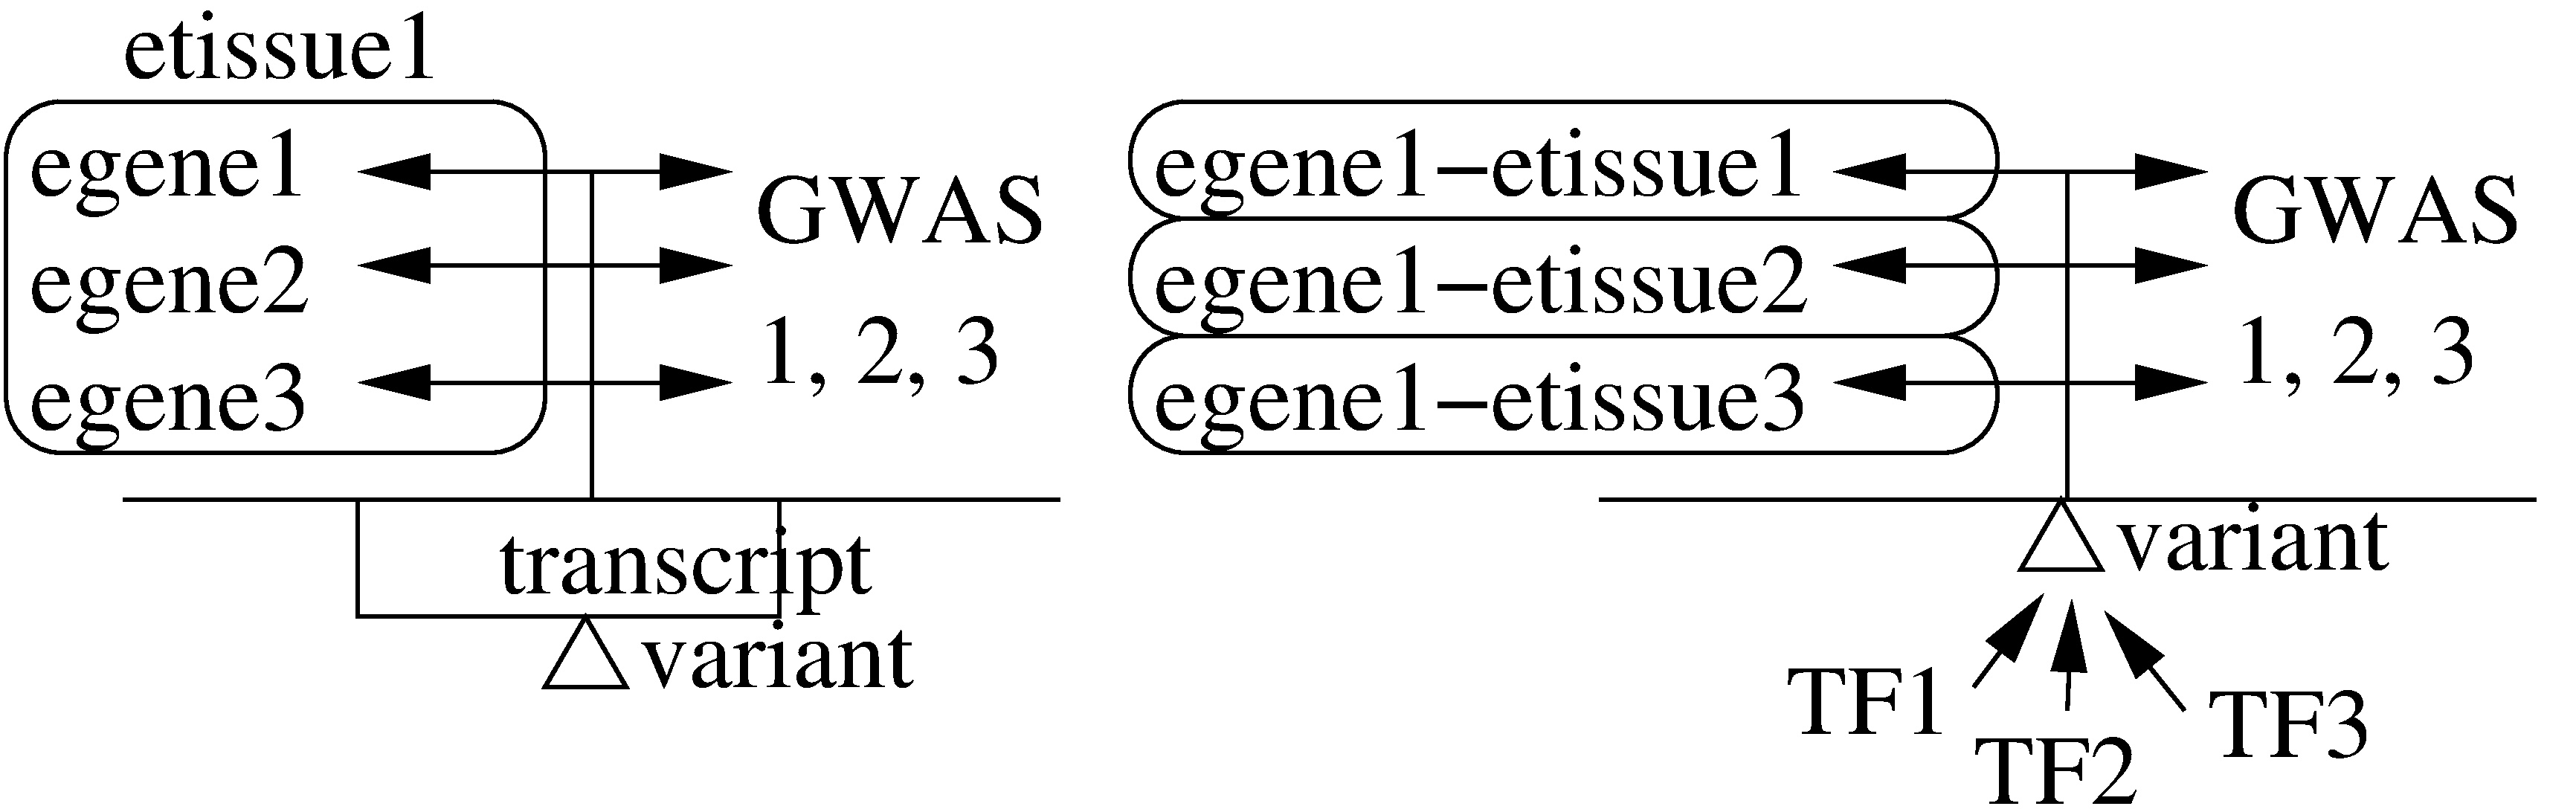
\includegraphics[width=\textwidth]{fig/graphical_summary.png}
\end{subfigure}

\caption{\textbf{Model of regulatory variant pleiotropy.} I have investigated three possible mechanisms of pleiotropy. \textbf{Left}, Pleiotropic variants have more eGenes that result in more functions and more phenotypes. This might arise from an enrichment of pleiotropic variants in splicing or 3' UTR regions. \textbf{Center}, I have also found that eGenes of pleiotropic variants are active in more etissues which result in more GWAS phenotypes. This might be explained from variants being bound by more transcription factors. \textbf{Left} Triplets of variant-eGene-eTissues are associated with more GWAS phenotypes, which directly affect the number of GWAS phenotypes. I have found that this might be explained by an enrichment of missense alleles.} \label{fig:beta}
%
\end{figure}

